\section{The Last Duel: God’s Justice}


\begin{quotex}
For the Lord is righteous, he loves righteous deeds.
\flright{\textsc{Psalm 11:7}}
\end{quotex}


\begin{wrapfigure}{rt}{.3\textwidth}
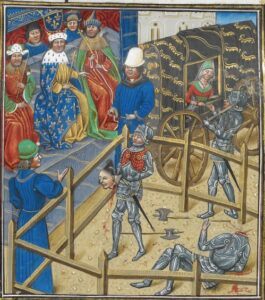
\includegraphics[width=.3\textwidth]{LastDeulImage-265x300.jpg}
\end{wrapfigure}

In the review of \textit{Gone, Baby, Gone}\footnote{See Section \ref{sec:GoneBabyGone} in this book.}, this question was raised: If the legitimate processes and procedures of the State do not result in justice in a particular case, is it appropriate for a citizen to bypass the State's system of justice?

In the recent film, \textit{The Last Duel}\footnote{\url{https://www.imdb.com/title/tt4244994/?ref\_=fn\_al\_tt\_1}}, a different question is raised: if the State's system of justice results in unresolvable aporia, how can justice be achieved?

\paragraph{Story}

The story tells of the 29 December 1386, trial by combat (duel) in which the Norman knight Jean de Carrouges dueled squire Jacques Le Gris. Carrouges had accused Le Gris of raping his wife, Marguerite, while he was away. It is based, rather closely, on actual events as they were documented in the subsequent trial of Jacques. The circumstances of the story can be found on Wikipedia, so we can focus on the trial itself.

\paragraph{Female Orgasm}


A common theory of the time was that pregnancy could result from intercourse only if the female experienced an orgasm. This notion has sources going back to Hebrew, Greek, and Roman times. Since rape was considered to be a great sorrow, a woman could derive no pleasure from it; hence rape could never result in pregnancy. I did an Internet search on the topic and discovered that many people hold the same belief today.

If you want my opinion, you should not rely on it as a method of birth control. It's like thinking you won't get fat if you don't enjoy the food.

\paragraph{The Trial}


Although there were a few minor witnesses, the main part of the trial consisted on the testimonies of Jean, Jacques, and Marguerite. Those of Jean and Jacques were documented, but Marguerite's was a fictional reconstruction because a woman's testimony was not considered reliable in court.

Keep in mind that the accusation was high risk for Marguerite. If Jacques were to be found innocent, then she would be burned alive for perjury in a rape case. That law might discourage frivolous sexual assault accusations.

\subsubsection{Jean de Carrouges}


Jean had to speak for his wife. He described his relationship with Jacques, their disputes, and subsequent reconciliation. Of course, the reconciliation is over since Jean believes his wife. While he was away on an errand, he asked his mother to never leave Marguerite alone. Nevertheless, the mother did leave her alone when she took all the servants for an errand of her home.

At the time, Jacques visited Marguerite, forced his way inside the house, and then allegedly raped her.

\subsubsection{Jacques Le Gris}


Jacques worked his way up to his position through his skills in accounting and business. He had a reputation as a womanizer and engaged in orgies. When he met the beautiful Marguerite at a public event, he assumed she was making goo-goo eyes at him. He admitted to visiting Marguerite where he expressed his undying love for her. He then chased her up to her chambers and took her on her bed.

He even admitted that she resisted his advanced, but, in his mind, women often feigned protests even though they secretly desired to be taken. After the deed, he warned her not to tell her husband.

\subsubsection{Marguerite}


Marguerite's testimony (fictionalized) did not add anything new. She denied misleading Jacques and insisted that the rape was real. Since she was pregnant, the question of paternity arose. The believed in the science of the time that the rapist could not be the father. However, paternity could not be determined one way or the other. Since she never conceived a child with Jean, the suspicion was that Jacques was the father. In that case, there was no rape since she derived pleasure from the act.

Ultimately, the case could not be resolved one way or another by the court.

\paragraph{The Duel}


Jean insisted on a legally sanctioned duel to finally salvage his wife's honor. This was granted to him. For the legal justification for the decision, see \textit{The Metaphysics of Dueling}\footnote{\url{https://gornahoor.net/?p=3636}}.

The duel itself was brutal. Although Jean was the older man, he had more battle experience. When he eventually got Jacques in a ``tap out'' position\footnote{\url{https://dictionary.cambridge.org/us/dictionary/english/tap-out}}, he demanded the latter's confession. Jacques, however, repeated his innocence. At that point, Jean killed him, which everyone accepted as a sign of Marguerite's purity.

If God is indeed righteous, how else do you resolve a ``he said, she said'' scenario. We often witness evil defeating the righteous, but battle, under those circumstances, do not meet Dante's criteria for a just duel. In any case, that was the last time that a duel was used in France to determine the outcome of a legal proceeding.

\paragraph{References}


From the Smithsonian magazine: The True History Behind `The Last Duel'\footnote{\url{https://www.smithsonianmag.com/history/the-true-history-behind-the-last-duel-180978860/}}.

For the history of the science of the female orgasm: Bitenosh's Orgasm, Galen's Two Seeds and Conception Theory in the Hebrew Bible\footnote{\url{https://brill.com/view/journals/dsd/28/1/article-p38\_3.xml?language=en}}.

\url{https://www.youtube.com/watch?v=mgygUwPJvYk} 

\flrightit{Posted on 2022-01-30 by Cologero}

\begin{center}* * *\end{center}

\begin{footnotesize}
\begin{sffamily}
\texttt{James on 2022-01-30 at 23:33 said:}

I also watched this movie and was mildly intrigued by it . I wonder if there was a possibility of satisfying the Dantean qualifications for a righteous duel by instead choosing champions of Emperor-esque quality , i.e. if it were possible to create a warrior-religious caste that would fight on behalf of all severe cases . ``public defenders'' so to speak . In other words , analogous to how lawyers are employed nowadays as officers of the court and abide by court ethics (in theory) and are experts on the law since the defendant and accuser are unable to attain that level of ``knowledge'' , what if it were possible to create an ORDER which fulfills this role on a spiritual level . Warrior-monks who take on cases as a means of coming together in fraternal mortal combat against each other for the sake of finding the Divine truth . This would sidestep the personal gains , hatred, or common lack of spirituality of the contestants and instead , for matters of grave purpose , the Lady may find her true champion and the gentleman may find his champion . If the warrior-monk in his judicial wisdom refuses to take up the cause of one of the parties , that in itself could be seen as indication enough that the cause is not just . It may be an interesting science fiction conceit I may have to explore for the future .

\end{sffamily}
\end{footnotesize}

